\section{Accomplishments}
%II.	ACCOMPLISHMENTS: Mandatory
%What was done? What was learned?
%The information provided
%in this section allows the agency to assess whether satisfactory progress has 
%been made during the reporting period. The PI is reminded that the grantee is 
%required to obtain prior written approval from the Contracting Officer 
%whenever there are significant changes in the project or its direction. 
%Requests for prior written approval must be submitted to the Contracting 
%Officer (submission via Fedconnect is acceptable).
%Summary recent work here.


\subsection{Goals}
%a.	What are the major goals of the project?
%List the major goals of the project as stated in the approved application or as approved by the agency. If the application lists milestones/target dates for important activities or phases of the project, identify these dates and show actual completion dates or the percentage of completion.
%Generally, the goals will not change from one reporting period to the next. However, if the awarding agency approved changes to the goals during the reporting period, list the revised goals and objectives. Also explain any significant changes in approach or methods from the agency approved application or plan.
The main goals and objectives of the project are:
\begin{itemize}
\item Make the automatic solver selection technology applicable to a broad range of nuclear reactor simulations by enabling solver selection throughout the spectrum of NEAMS tools. 
\item Extend the automatic solver selection to a special category of numerical subproblems (physics based preconditioning, matrix free methods etc.) and leadership platforms that are important to NEAMS applications. 
\item Investigate other performance objectives such as accuracy, resiliency, and energy efficiency for optimal solver selection in addition to CPU time. Cater to a wide range of simulation problems and customers with varying performance criteria. 
\item Integrate the above techniques into a pluggable software API and Library that can be leveraged in codes developed by NEAMS. Design and implement the software indirections that will enable plug-n-play integration of the proposed features into other numerical software.
\end{itemize}

The overall view of the proposed framework is outlined as shown in Figure 1. The major technical goals of the project will be accomplished by executing the  list of technical tasks as stated in the proposal:
\begin{itemize}
\item[Task 1:] Automatic Solver Selection for Fuels Product Line: Code instrumentations and data collections on MOOSE and BISON problems.
\item[Task 2:] Automatic Solver Selection for Reactors Product Line: Examination of problems that can benefit from this approach in Diablo and SHARP problems. 
Extending automatic solver selection approaches to the reactors product line. 
\item[Task 3:] Matrix Free methods: Development of new approaches for matrix free methods. Develop novel methods for partial Jacobian and physics based preconditioning.
\item[Task 4:] Other Performance metrics: Evaluate automatic solver selection 
algorithms and its impact in terms of efficiency gain (CPU time), accuracy, 
energy efficiency, and resilience of overall NEAMS simulations.
\item[Task 5:] Multi-objective Optimization: Incorporate optimization of multiple 
objectives into the solver modeling and selection framework.
\item[Task 6:] Optimizations Targeting DOE Computing Facilities: Training data for 
Machine Learning models will be built using compute infrastructure at DOE labs.
\item[Task 7:] System Integration and Software Indirections: Integration of all 
features into a unified framework.
\end{itemize}

\begin{figure}
 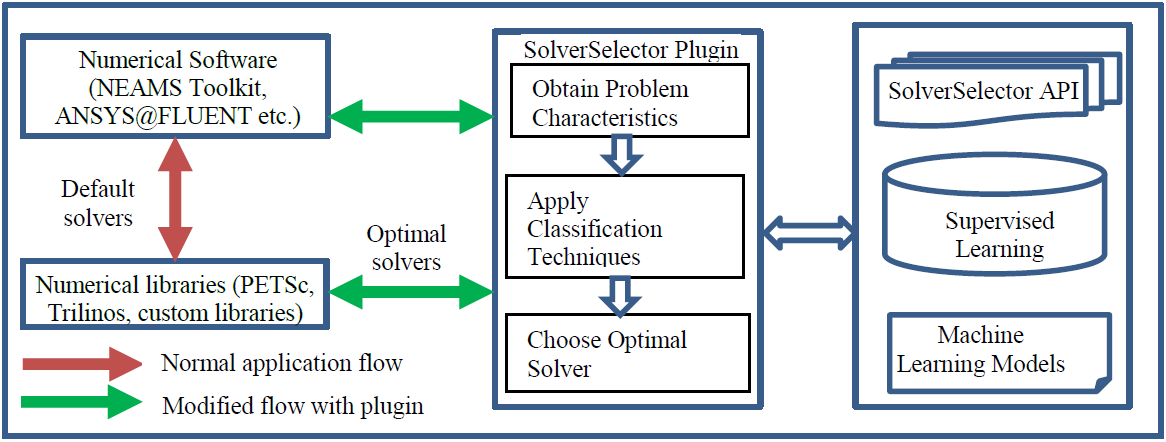
\includegraphics[width=\textwidth]{figures/proposed_framework.png}
  \caption{ Overview of intended use of the proposed plugin.\label{fig:overview} }
 \end{figure}


\subsection{Recent Accomplishments}
The report will outline relevant work carried out in the 6 month period December 2017-May 2018. During this reporting period, the project team continued to focus on Tasks 2, 3 and 7. 

\subsection{Task 2: Automatic Solver Selection for the Reactors Product Line}

The NEAMS reactor product line consists primarily of PROTEUS, Nek5000 and Diablo physics codes. Among these, both Nek5000 and PROTEUS developed at ANL, have been shown to strong scale well (over 512K processes) on HPC architectures. 

During this reporting period the project team continued its work related to extracting relevant and meaningful training data from the PROTEUS line of tools. This involved equipping the Proteus software with the necessary software indirections and interfaces for dumping the petsc-based linear solver matrices to file, as well as obtaining run-time logs of the linear solver. The modified Proteus software was then used to extract the matrices and solver performance information from a range of simulations using the Proteus benchmark problems. 

The data obtained from these simulations will be fed into our machine learning algorithms in the upcoming reporting period. This will allow the project team to explore the effects domain specific features have on the accuracy of the machine learning algorithm, ultimately allowing us to develop tools and techniques for developing a robust machine learning algorithm for individual tools such as those in the NEAMS toolkit. The project team have also begun work to set up several larger, real-world Proteus simulations to further aid in this research. The results from these larger simulations are expected in the upcoming reporting period. 


\subsection{Task 3: Matrix Free Methods}  

A large majority of MOOSE based applications, including BISON and MARMOT, use matrix-free methods to solve
the linear systems. Rather than storing the coefficient matrix explicitly, matrix-free methods access the matrix by evaluating matrix-vector products. This poses a difficulty for automatic solver selection because the majority of the classification features, i.e, the matrix norm, the trace and the row variance, require direct access to the matrix co-efficients.  The extraction of features from systems defined using a matrix-free approach is cutting-edge and novel research. During this reporting period, the project team developed a sampling based technique for matrix-free feature extraction that has proven to be very successful. This is a very promising result as it extends the domain of the solver selection algorithm to include matrix-free nonlinear solvers such as the Preconditioned Jacboian Free Newton Krylov method (PJFNK) favored in MOOSE. 

The development of the sampling based approach came after a detailed evaluation of a range of matrix-free feature extraction techniques that used only matrix-vector multiplications to extract features. This included an investigation into the three methods outlined in the previous progress report. Those methods included using a graph coloring algorithm to extract matrix values, an incomplete power iteration to estimate the eigenvalues, and a stochastic method for estimating the trace and the row variance. Each of those methods were tested and subsequently disregarded for being either to inaccurate (stochastic trace and row variance), to expensive (graph coloring) or, ineffective (incomplete power iteration). In contrast, the sampling based approach provided a good balance between accuracy and computational cost. 

\subsubsection{Sample Based Matrix-free Feature extraction}

Define a $n\times n$ matrix A with columns $\mathbf{a}_j$ such that  
\[ A = 
\begin{bmatrix}
    \vert & & \vert \\
    \mathbf{a}_1   & \dots &\mathbf{a}_n   \\
    \vert & & \vert
\end{bmatrix},
\]   

Then, one can extract the vector $\mathbf{a}_j$ through a single matrix-vector multiplication with the $j'th$ Euclidean basis vector. That is to say, 

\[ \mathbf{a}_j = A \mathbf{e}_j \] where $\mathbf{e}_j = \{0,0,\dots,1,0\dots\}$ represents the $j$'th standard basis vector. In fact, one can determine the effective value of each and every element in a $n \times n$ matrix-free system using at most $n$ matrix-vector multiplications. However, this is an O($n^3$) approach that returns optimal results in terms of feature accuracy, but is to expensive for use in a practical setting.

Our approach has been to use a small O(1) sample of the matrix columns to inform estimates of overall matrix features. Let $S$ represent a set containing $m \ll n $ columns of A. Then, the set $S$ can be formed in a matrix-free environment through the use of $m$ matrix-vector multiplications at a cost of O($mn^2$).  

To ensure accuracy and to minimize bias, it is essential that the sample set $S$ encompasses a good cross-section of the columns in $A$. This is particularly true for the matrices that arise from grid based PDE methods. In those cases, each column of $A$ represents a point in the computational grid. As such, features such as boundaries can dramatically effect the size and number of elements in rows. To that end, it is advantageous to select a sample that includes a good mix of columns linked to interior and boundary based grid points. In fact, our testing has shown that it is beneficial to pick and choose which sample columns are used in each feature calculation. For example, due to the effects of boundary conditions on the contents of some columns, it is best to use columns that translate to interior mesh points to the estimate the number of non-zeros in the matrix. Various other features make similar decisions, using different subsets of the overall sample data to calculate the final value.

Another important aspect of the sample based feature extraction technique is the statistical scaling of the features. Where appropriate, all features calculated are scaled by the ratio $n/m$ to ensure that the feature calculations reflect estimates of the overall matrix rather than just the sample set. Some features, such as those including maximums or minimums, do not use scaling, but instead assume that the value calculated using the sample set is representative of the entire matrix.   

Table~\ref{ffs} outlines the features that we were able to calculate using this approach. The Sample column notes the subset of the data that was used to calculate that feature as explained above. One of five subsets were used; (1) full: the full sample data set, (2) interior: Only columns representing interior grid points (3) boundary: Only columns representing boundary grid points were used, (4) square: Only the elements $A_{ij}$ for ${i,j} \in S$\footnote{This forms a square, $m\times m$ sub-matrix that can be tested for properties such as symmetry}.  Features that were scaled are marked with a $^*$.



\subsubsection{Implementation Details} 

The primary concern for automatic solver selection, both in the matrix-free and standard matrix based systems is that the cost of feature extraction acts to counteract the time saving benefits of choosing the optimal solver. Certainly, in situations where the best solver is already known, the cost associated with feature extraction will actually cause the method to be slower. Likewise, in situations where a poor default solver is used, the cost of feature extraction will be negligible when compared to the run-time reduction obtained by using the optimal solver. 

As such, it is essential that the feature extraction techniques be as efficient as possible. To ensure this, the matrix-free feature extraction routine has been implemented directly in Petsc using a single loop. That is to say, for each column in the sample set, we complete a single matrix vector multiplication, followed by a single loop through the values of the column. If multiple cores are used, this is completed in parallel, with the only communication between processors being completed during the matrix-vector multiplication as required by Petsc. 

A single MPI Reduce call is made at the completion of the feature extraction stage, at which point the root processor completes the final collation and calculation of the matrix-free features. In a practical setting, the root processor would then feed those features into the machine learning algorithm before scattering back the details of the optimal solver to the remaining processors. 

This computation-then-communication pattern is extremely efficient in terms of latency, but is somewhat bandwidth heavy. For example, the entire square data set ($m^2$ elements, where $m$ is the number of samples) must be sent through to the root process so that the symmetrical features can be calculated. Given that we require $m$ to be small, we do not foresee this being a problem because, in cases where the need for a large $m$ arises, the cost of the $m$ matrix-vector multiplications, both in terms of time and memory, will likely overshadow any costs associated with the high bandwidth MPI Reduce call.  

\subsubsection{Results}

In the following tests we highlight some results of our matrix-free feature extraction algorithms. To ensure we can check and verify our results, real matrices with known matrix-values were used. These matrices were obtained from the Florida sparse matrix collection. Note that there is no algorithmic difference between using the matrix-free feature extraction techniques on a matrix in which the matrix elements are known, and in a matrix-free system where only the action of the matrix on a vector is available \footnote{ In the case that the elements are known, one could reduce the computational cost by simply extracting the sample columns from memory, however, we chose to complete the matrix-vector multiplications to ensure the performance results are representative of a real-world matrix-free problem.} All of the following tests were performed on a linux based virtual machine ( Windows host) using a single processor and a standard hp Desktop. Parallel tests using RNETs multi-node cluster are planned for the upcoming reporting period.  

Figures~\ref{accuracy0}-\ref{accuracy3} plot the error in four of the matrix-free features against the number of non-zeros in the matrix for every matrix in our database. Each figure presents the accuracy for a different sample set $S(i,e)$, where $e$ indicates the number of boundary columns used  and $i$ indicates the number of interior point columns. In this case, the interior columns were selected randomly while the boundary columns were chosen to be columns $0$ to $\lfloor e/2 \rfloor $ and $n-\lfloor e/2 \rfloor $ to $n$. The error in a feature is defined to be the difference between the exact and calculated feature value divided by the magnitude of the exact feature value. The four features presented where chosen because they were deemed to be important features in our previous tests for standard matrix based systems. 

\begin{figure}[h]
    \centering
    \begin{subfigure}{0.475\textwidth}
     \centering 
     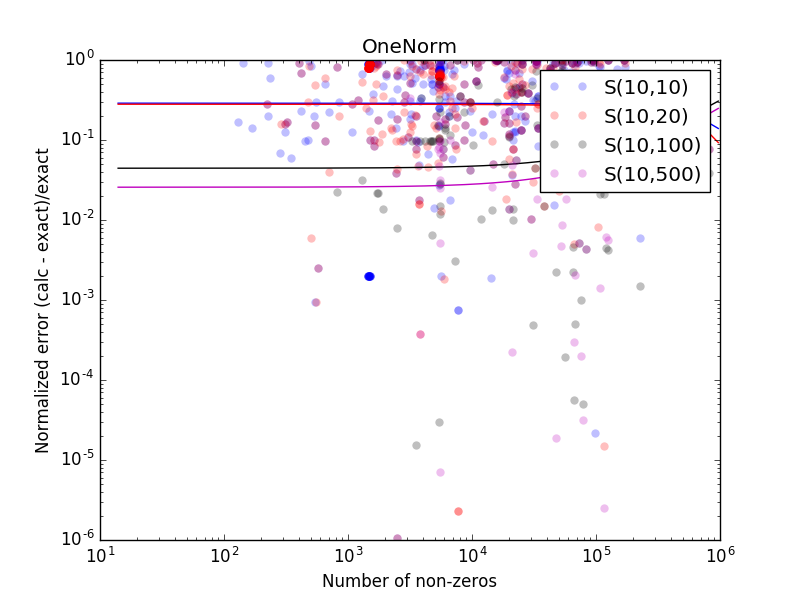
\includegraphics[width=\textwidth]{figures/figure1.png}
     \caption{One Norm }
     \label{accuracy0}
     \end{subfigure}
     \hfill
    \begin{subfigure}{0.475\textwidth}
     \centering 
     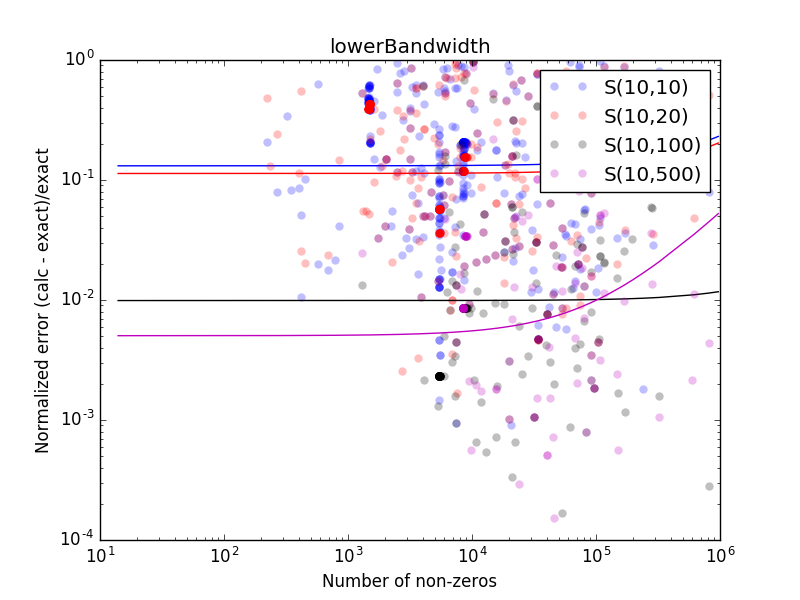
\includegraphics[width=\textwidth]{figures/figure2.png}
     \caption{Lower Bandwidth}
     \label{accuracy1}
     \end{subfigure}
     \vskip\baselineskip
     \begin{subfigure}{0.475\textwidth}
     \centering 
     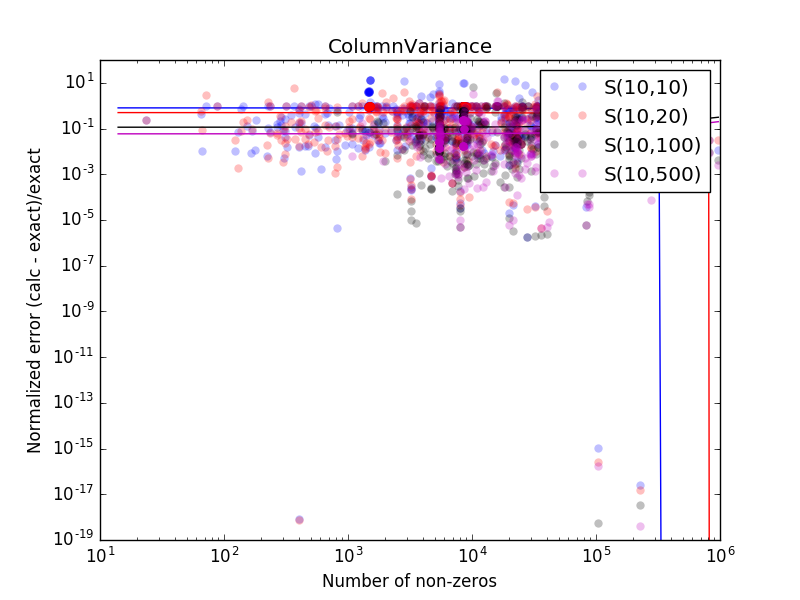
\includegraphics[width=\textwidth]{figures/figure3.png}
     \caption{Column Variance}
     \label{accuracy2}
     \end{subfigure}
     \hfill
     \begin{subfigure}{0.475\textwidth}
     \centering 
     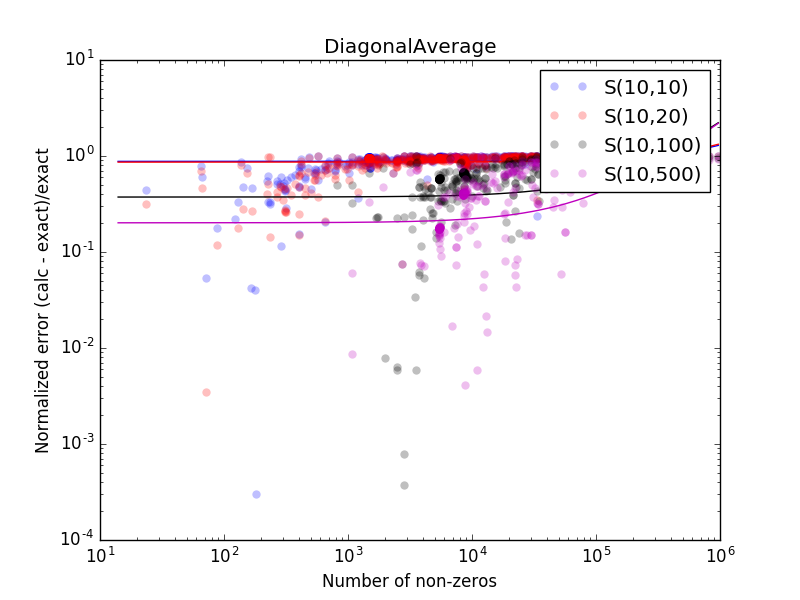
\includegraphics[width=\textwidth]{figures/figure4.png}
     \caption{Diagonal Average}
     \label{accuracy3}
     \end{subfigure}
     \caption{ The normalized error four four of the features when calculated with using the matrix-free sampling approach. Each marker indicates a different matrix. The solid lines represent a the linear line of best fit through the data obtained for each sample set. Both the x and y axis are presented using a log scaling due to the large differences in values. }
\end{figure}

The important thing to note here is that the error increases as the sample size decreases.  If one chooses to sample all rows, the feature set is 100\% accurate, with the accuracy decreasing from there as the sample size drops. 

\begin{figure}[h]
    \centering
    \begin{subfigure}{0.475\textwidth}
     \centering 
     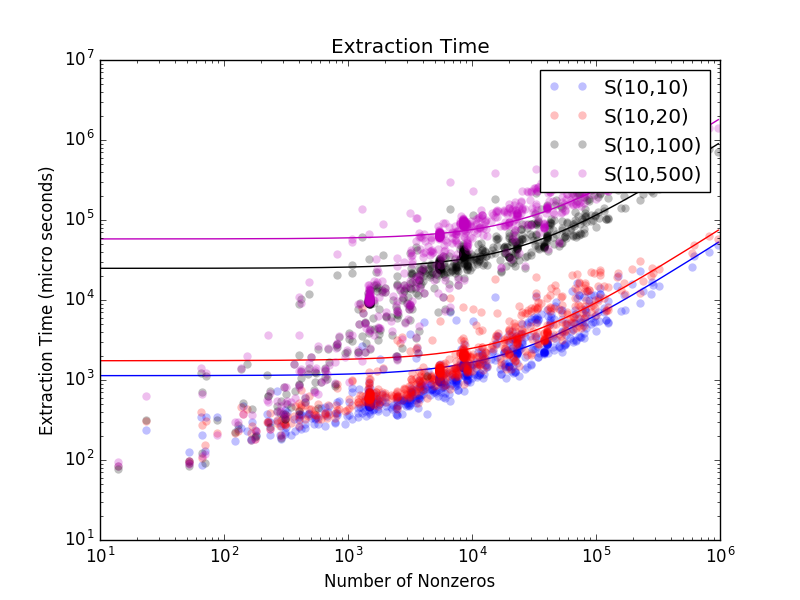
\includegraphics[width=\textwidth]{figures/figure5.png}
     \caption{Time required to extract feature plotted against number of non zeros for matrices in the moose dataset. }
     \label{3accuracy0}
     \end{subfigure}
    \hfill
    \begin{subfigure}{0.475\textwidth}
     \centering 
     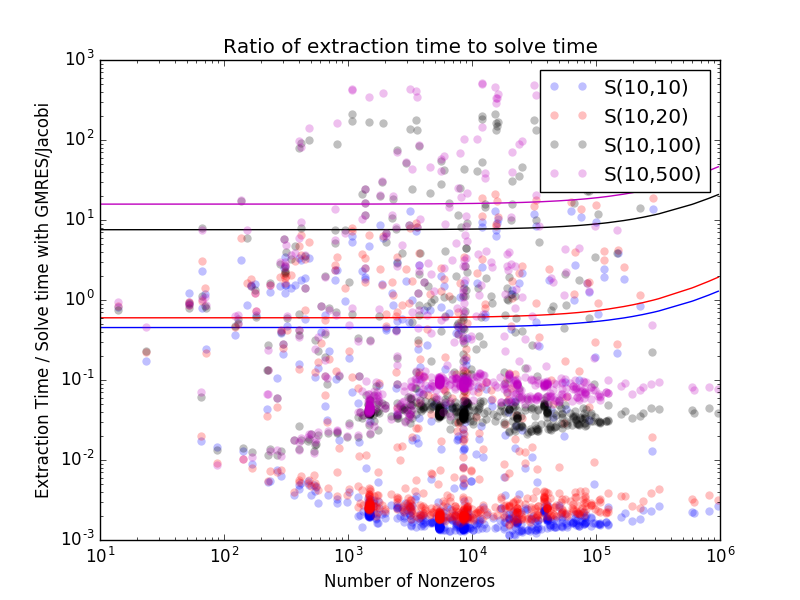
\includegraphics[width=\textwidth]{figures/figure6.png}
     \caption{Time required to extract feature over the time required to solve the system using GMRES preconditioned with ILU plotted against number of non zeros for the matrices in the moose dataset. }
     \label{3accuracy1}
     \end{subfigure}
\end{figure}


Another important aspect of feature extraction is the cost. Figure~\ref{3accuracy0} plots the time taken to extract the entire set of features against the number of non-zeros for the entire matrix data set, for the set of randomized sample-sets used in Figures~\ref{accuracy0}. Figure~\ref{3accuracy1} takes this a step further, plotting the ratio of feature extraction time over the time taken to solve the matrix using GMRES preconditioned with Jacobi. GMRES preconditioned with Jacobi can be used to solve a wide range of problems, although Jacobi is not generally thought of as a fast preconditioner, with many better, albeit less robust, options available.  

Based on these figures it is clear that reducing the size of the feature set also reduces the cost. This should not be surprising as a smaller sample set means less matrix-vector multiplications, less data to process and a smaller memory requirement. Most importantly, for the majority of the matrices, the time taken to extract the features was much less than the solve time. This is extremely promising indicating that large run-time reductions should be possible in real world situations. 

One final approach for reducing the cost of feature extraction is to reduce the number of features in the feature set, with the downside being that reducing the number of features will likely reduce the effectiveness of the machine learning models. A similar approach was used for standard matrix-based systems with good results. Table~\ref{reduced_sets} shows the features included in the reduced feature sets found for standard matrix based systems. Figures~\ref{4accuracy0}-\ref{4accuracy1} plot the time required to extract the features for the full and reduced feature sets for four different sample sets. Interestingly, there is little to no difference between the time taken to extract the features when the sample size is small. However, once the sample size increases, the differences become quite large. 

\begin{table*}[thb]
\centering
\caption{Matrix-free: Reduced Feature Sets}
\label{reduced_sets}
\begin{tabular}{|c|c|c|}    \hline  
Features                   & Reduced Set 1  & Reduced Set 2 \\ \hline\hline
Min. Non zeros/row         & X              & X             \\ \hline
Lower Bandwidth            & X              & X             \\ \hline
NonZeroPatternSymmetryV1   & X              &               \\ \hline
Infinity Norm              & X              &               \\ \hline
Column Variance            & X              & X             \\ \hline
Diagonal Non Zeros         & X              & X             \\ \hline
Diagonal Average           & X              & X             \\ \hline
\end{tabular}
\end{table*}

\begin{figure}[h]
    \centering
    \begin{subfigure}{0.475\textwidth}
     \centering 
     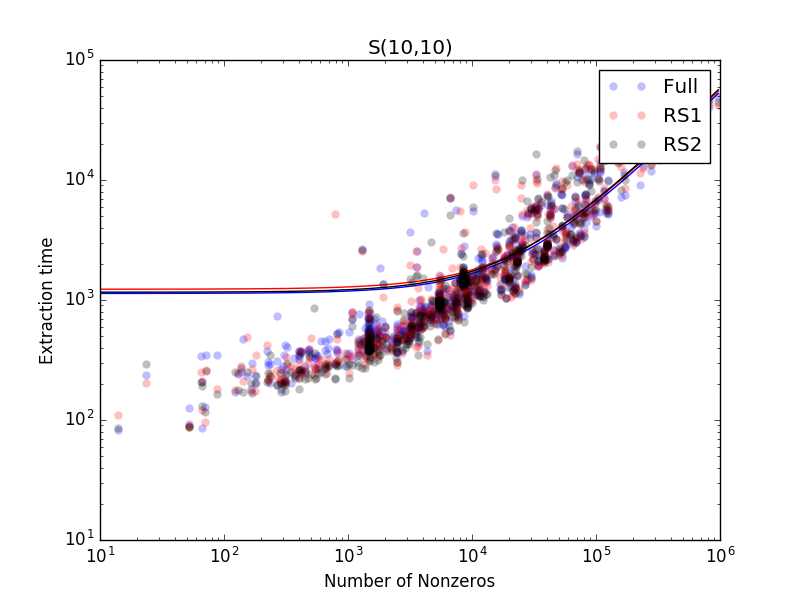
\includegraphics[width=\textwidth]{figures/figure7.png}
     \caption{ $S(10,10)$ }
     \label{4accuracy0}
     \end{subfigure}
     \hfill
    \begin{subfigure}{0.475\textwidth}
     \centering 
     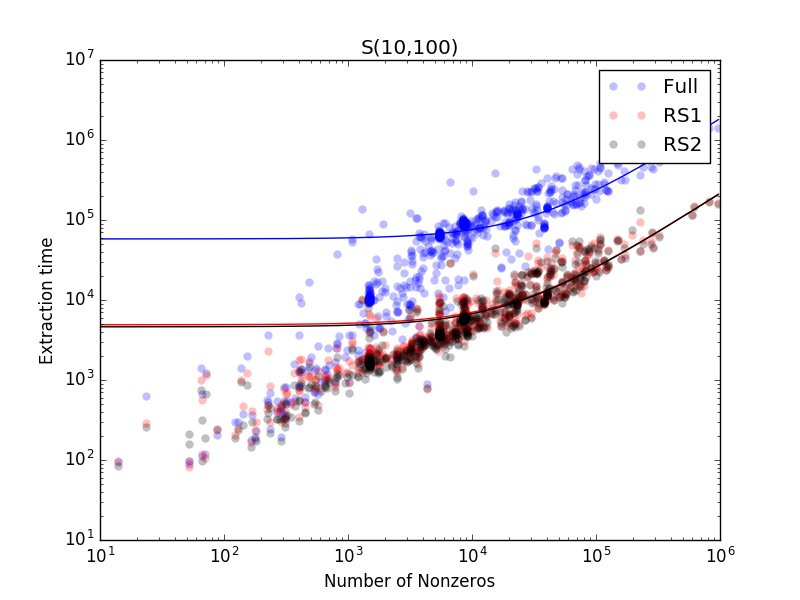
\includegraphics[width=\textwidth]{figures/figure8.png}
     \caption{$S(10,100)$}
     \label{4accuracy1}
     \end{subfigure}
     \caption{Time required to extract the features in each feature set for two different sample sets.}
\end{figure}

All in all, these results show that, when carefully tuned, the sample based feature extraction method developed and implemented during this reporting period is more than capable of producing an accurate set of features at a cost that is small when compared to a basic Krylov solver. The next step is to determine the effectiveness of each feature set. That is, how good are the machine learning models at classifying solvers when trained and tested using these feature sets. The project team is currently running these tests with results expected within the first month of the next reporting period; however, early results using a matlab implementation of the extraction algorithm have produced models with between 90 and 100\% overall accuracy depending on the learning algorithm used. 

\subsection{ Task 7: SolverSelector API }
\label{API}
Task seven addresses the issue of developing the software indirections that allow for plug-and-play integration of the solver selector features into the NEAMS solvers. During this reporting period, the project team continued the development of it SolverSelector API. 

In particular, the project team focused on integrating the aforementioned matrix-free feature extraction techniques into the petsc interface of the API. While the API is designed to be applicable to a variety of linear solver apckages, Petsc was chosen for testing and development because it is a mature framework that supports a wide range of Krylov solvers and practitioners. Moreover, Petsc is used widly across the numerical simulation community and is the go to tool when it comes to krylov based linear solvers. In particular, the MOOSE framework, and hence a large number of NEAMS tools, use Petsc for its linear algebra and linear solver algorithms. 

As of the end of this reporting period, the Solver selector API allows the user to:
\begin{itemize}
 \item Build a machine learning database using matrices stored in the Petsc binary format using a simple input file format. 
 \item Extend the machine learning database at run-time through the use of a simple input file format. This is particularly useful for matrix-free methods, where one cannot build the database externally using saved matrix files. 
 \item Use machine learning to automatically select the best linear solver based on a pre-built machine learning database and model (i.e., online linear solver optimization)
 \item Perform cross-validation testing to access the validity and accuracy of the machine learning model based on the current database
 \item Save the optimal solver choice for use at a later point, increasing efficiency for problems where the matrix values do not change dramatically between runs or linear solves (i.e., offline linear solver choice optimization).
\end{itemize}

The project team has integrated and used each of these features in both matrix-free and standard matrix systems from both the Petsc and Moose example sets. In both cases, utilizing the solver selection features requires less than five lines of additional code and two command line parameters. 

\subsection{Training and Professional Development}

This project has provided opportunities for research development and collaboration with Dr. Boyana Norris at The University of Oregon (UO). The UO subcontract includes the support of graduate students. We are also closely working with Dr. Vijay Mahadevan from Argonne National Laboratory who is interacting with the Diablo team and also looking at PROTEUS to generate relevant operators for problems of interest.
%c.	What opportunities for training and professional development has the project provided?
%Describe opportunities for training and professional development provided to anyone who worked on the project or anyone who was involved in the activities supported by the project. .?Training? activities are those in which individuals with advanced professional skills and experience assist others in attaining greater proficiency. Training activities may include, for example, courses or one-on-one work with a mentor. ?Professional development? activities result in increased knowledge or skill in one?s area of expertise and may include workshops, conferences, seminars, study groups, and individual study. Include participation in conferences, workshops, and seminars not listed under major activities.

\subsection{Dissemination}
Currently, the work is in the development phase. Once completed, we will leverage our contacts in various National Laboratories and Government Agencies to demonstrate our SolverSelector plugin and the performance benefits, among others. The ultimate plan is to develop and commercialize a flexible automatic solver API. A research paper based on the matrix-free feature extraction techniques and the associated machine learning models is being written by our collaborators in Oregon for submission to the Copper Mountain special issue of SISC. 
%d.	How have the results been disseminated to communities of interest?
%Describe how the results have been disseminated to communities of interest. Include any outreach activities that have been undertaken to reach members of communities who are not usually aware of these research activities, for the purpose of enhancing public understanding and increasing interest in learning and careers in science, technology, and the humanities.

\subsection{Plans}
%e.	What do you plan to do during the next reporting period to accomplish the goals?
%Describe briefly what you plan to do during the next reporting period to accomplish the goals and objectives.
In the upcoming no cost time extension period, the Solver selector API will be hardened, tested, documented and extended. However, the majority of the work will be focused on improving the underlying machine learning models; a task that will be made much easier through the solver selector API. This will include detailed testing and analysis of our run-time solver selection algorithms in real-world examples starting with the examples in Petsc and Moose and moving up through to examples using NEAMS tools such as PROTEUS and BISON. Impressive run-time reductions for these simulations, especially in the matrix-free case, will be a key selling point for the Solver Selector API. 

In addition to this, the project team will begin to investigate some of the additional features and algorithms outlined in the no-cost-time-extension request, such as a model for extrapolating training data obtained using a small number of processors for use on large-scale compute resources. Building the training data sets is expensive, hence these extrapolation techniques and algorithms will extremely useful in removing the computational burden associated with setting up the machine learning models. 

\begin{table*}[htb]
\scriptsize
\caption{Full Feature Set}
\label{ffs}
\resizebox{\linewidth}{!}{%
\begin{tabular}{|p{3.2cm}|p{7.8cm}|p{1cm}|}    \hline  

Features                   & Description   & Sample Set  \\ \hline \hline
Dimension                  &    This feature gives the size of the matrix $A$. For a square matrix, the matrix size is the number of rows or columns of the matrix. & \\ \hline 
Number of non-zeros $^*$        &    The total number of non zeros in the coefficient matrix $A$. & interior \\ \hline 
Minimum non-zeros per row  &    This property finds the minimum number of non zeros in any row of the matrix $A$. & boundary \\ \hline 
Maximum non-zeros per row  &    This feature gives the maximum number of non-zeros in any row of the matrix $A$. & interior \\ \hline 
Average non-zeros per row $^*$ &    This feature provides the average number of non-zeros per row for the matrix $A$. & full \\ \hline 
Row diagonal dominance     &    This feature computes the row diagonal dominance of the matrix $A$. It returns $0$ if its not diagonally dominant. & full \\  \hline 
Symmetricity               &    This feature finds whether the matrix is symmetric or not. For a matrix to be symmetric, it is equal to its transpose ($A = A^{T}$). & square \\ \hline 
Trace  $^*$                    &    This feature computes the sum of the elements of the main diagonal of the matrix $A$. & full \\ \hline 
Absolute Trace  $^*$           &    This feature computes the sum of absolute values of the diagonal elements of the matrix. &  full \\ \hline 
Diagonal non-zeros $^*$        &    This feature counts the number of non-zero elements on the diagonal. & full\\    \hline 
One norm   &    This feature gives the maximum column sum of the matrix $A$. It is denoted by the formula     $||A||_{1} = max_{j} \sum |A_{ij}|_{i=1}^{m}$, where $j=1, \ldots, m$. & full \\ \hline 
Infinity norm              &    The infinity norm is computed as follows: $||A||_{\infty} = \max (\sum_{j=1}^{n} |A_{1 j}|, \sum_{j=1}^{n} |A_{2 j}|, \ldots, \sum_{j=1}^{n} |A_{m j}|)$ & full \\ \hline 
Symmetric Infinity norm    &  This feature provides the infinity norm of only the symmetric part of the matrix $A$. &square \\ \hline 
Anti symmetric Infinity norm    &    This feature computes the infinity norm of the anti-symmetric part of the matrix $A$. & square \\ \hline 
Frobenius norm  $^*$           &    This feature gives the square root of the sum of the absolute squares of its elements. It is denoted by $\sqrt{\sum_{i=1}^{m} (\sum_{j=1}^{n} |A_{ij}|^2})$. & interior \\ \hline 
Symmetric Frobenius norm $^*$  &    Frobenius norm of the symmetric part of the matrix. & square \\ \hline 
Anti symmetric Frobenius norm $^*$  &    This feature gives the Frobenius norm of the anti-symmetric part of the matrix. & square \\ \hline 
Absolute non-zero sum  $^*$    &    Sum of the absolute values of all the non- zeros in matrix. & interior \\ \hline 
Diagonal Average $^*$          &    This feature computes the average of the absolute values of the diagonal elements of a matrix. & full \\ \hline 
Lower Bandwidth            &    The smallest number k, such that any entry $a_{i,j} = 0$ when $i - j \textgreater k$. & full \\ \hline 
Upper Bandwidth            &     The smallest number k, such that any entry $a_{i,j} = 0$ when $j \textgreater i + k$. & full \\ \hline 
Average diagonal distance $^*$ &    This feature gives the average distance of nonzero diagonal to the main diagonal. & interior \\ \hline 
Non zero pattern symmetry V1   &    Checks the nonzero pattern symmetry. If symmetric, returns 1 otherwise 0. & square \\ \hline 
Column diagonal dominance  &    This feature computes the column diagonal dominance of the matrix. It returns 1 if it is diagonally dominant, and 0 otherwise. & full \\ \hline 
Diagonal sign              &    This feature indicates the diagonal sign pattern of the matrix. The value is -2 for all negative elements, -1 for some non-positive elements, 0 if all elements are zero, 1 is some elements are non-negative, 2 if all elements are positive. & full \\ \hline 
Row variance               &   This feature computes the row variance of the matrix & interior \\ \hline 
Column variance            &   The feature computes the columns variance of the matrix & interior \\ \hline  
\end{tabular}}
\end{table*}

 
